\documentclass[a4paper, 10pt]{article}
\usepackage[utf8x]{inputenc}
\usepackage{graphicx}
\usepackage{geometry}
\usepackage{amsmath}
\usepackage{mathenv}
\usepackage{amssymb}
\usepackage{amsfonts}
\usepackage{mathrsfs}
\usepackage{textcomp}
\geometry{hmargin = 2.5cm, vmargin = 1.5cm}

% OPENING
\title{SY09 - TP04\\Analyses discriminantes quadratique et linéaire}
\author{Bertrand Bon - Antoine Hars}

\begin{document}

\maketitle

\section*{Introduction}
Dans le cadre de ce tp, nous avons étudié les analyses discriminantes quadratique et linéaire.\\ \\

\section*{Exercice 1 : Règle de Bayes.}
On suppose que la population est répartie en deux classes, en proportions $\pi_{1}$ et $\pi_{2}$ = 1 - $\pi_{1}$,
issues des distributions gaussiennes bivariées $\mathcal{N}(\mu_{1}, \Sigma_{1})$ et $\mathcal{N}(\mu_{1}, \Sigma_{1})$.\\

\subsection*{1. Donner une équation de la frontière de décision de la règle de Bayes dans chacun des cas suivants :}
Pour le calcul de ces équation de la frontière de décision de la \textbf{règle de Bayes} pour les cas suivants,
nous nous sommes basés sur les fonctions discriminantes.\\
Elles nous donnent, dans le cas des coûts {0, 1}, la \textbf{règle de Bayes} s'écrivant de la manière suivante :\\
$g$*(x) = $\omega_{k*}$ avec $k$* = arg $\underset{k}{max}$ $g_{k}$(x), avec\\
\begin{align*}
g_{k}(x) &= ln f_{k}(x) + ln \pi_{k}\\
 	 &= -\frac{1}{2}(x - \mu_{k})' \Sigma_{k}^{-1} (x - \mu_{k}) - \frac{1}{2} ln(det \Sigma_{k}) + ln \pi_{k} - \frac{p}{2} ln(2\pi)
\end{align*}
\subsubsection*{(a) $\pi_{1}$ = 0.5, $\mu_{1}$ = (0,0)´, $\mu_{2}$ = (1,1)´, $\Sigma_{1}$ = $\Sigma_{2}$ =
$\begin{pmatrix} 1 & 0 \\ 0 & 1 \end{pmatrix}$ :}
\begin{align*}
g_{1}(x) &= -\frac{1}{2} ((x_{1}, x_{2}) - (0, 0)')' \begin{pmatrix} 1 & 0 \\ 0 & 1 \end{pmatrix} ((x_{1}, x_{2}) - (0, 0)') -
\frac{1}{2} ln(1) + ln(0.5) - \frac{2}{2} ln(2\pi)\\
	 &= -\frac{1}{2} (x_{1}² + x_{2}²) + ln(0.5) - ln(2 \pi)\\ \\
g_{2}(x) &= -\frac{1}{2} ((x_{1}, x_{2}) - (1, 1)')' \begin{pmatrix} 1 & 0 \\ 0 & 1 \end{pmatrix} ((x_{1}, x_{2}) - (1, 1)') -
\frac{1}{2} ln(1) + ln(0.5) - \frac{2}{2} ln(2\pi)\\
	 &= -\frac{1}{2} ((x_{1} - 1)² + (x_{2} - 1)²) + ln(0.5) - ln(2 \pi)\\ \\
g_{1}(x) = g_{2}(x) &\Leftrightarrow (x_{1}² + x_{2}²) = (x_{1} - 1)² + (x_{2} - 1)² \Leftrightarrow x_{1} + x_{2} = 1
\Leftrightarrow x_{1} = 1 - x_{2}
\end{align*}\\

\subsubsection*{(b) $\pi_{1}$ = 0.1, $\mu_{1}$ = (0,0)´, $\mu_{2}$ = (1,1)´, $\Sigma_{1}$ = $\Sigma_{2}$ =
$\begin{pmatrix} 1 & 0 \\ 0 & 1 \end{pmatrix}$ :}
\begin{align*}
g_{1}(x) &= -\frac{1}{2} ((x_{1}, x_{2}) - (0, 0)')' \begin{pmatrix} 1 & 0 \\ 0 & 1 \end{pmatrix} ((x_{1}, x_{2}) - (0, 0)') -
\frac{1}{2} ln(1) + ln(0.1) - \frac{2}{2} ln(2\pi)\\
	 &= -\frac{1}{2} (x_{1}² + x_{2}²) + ln(0.1) - ln(2 \pi)\\ \\
g_{2}(x) &= -\frac{1}{2} ((x_{1}, x_{2}) - (1, 1)')' \begin{pmatrix} 1 & 0 \\ 0 & 1 \end{pmatrix} ((x_{1}, x_{2}) - (1, 1)') -
\frac{1}{2} ln(1) + ln(0.9) - \frac{2}{2} ln(2\pi)\\
	 &= -\frac{1}{2} ((x_{1} - 1)² + (x_{2} - 1)²) + ln(0.9) - ln(2 \pi)\\ \\
g_{1}(x) = g_{2}(x) &\Leftrightarrow  x_{1} = 1 - x_{2} - ln(9)
\end{align*}\\

\subsubsection*{(c) $\pi_{1}$ = 0.5, $\mu_{1}$ = (0,0)´, $\mu_{2}$ = (1,1)´, $\Sigma_{1}$ = $\Sigma_{2}$ =
$\begin{pmatrix} 1 & -0.3 \\ -0.3 & 1 \end{pmatrix}$ :}
\begin{align*}
\Sigma_{1}^{-1} &= \Sigma_{2}^{-1} = \frac{1}{0.91} \begin{pmatrix} 1 & 0.3 \\ 0.3 & 1 \end{pmatrix}\\
g_{1}(x) &= -\frac{1}{2} \frac{1}{0.91} ((x_{1}, x_{2}) - (0, 0)')' \begin{pmatrix} 1 & 0.3 \\ 0.3 & 1 \end{pmatrix}
((x_{1}, x_{2}) - (0, 0)') - \frac{1}{2} ln(1) + ln(0.5) - \frac{2}{2} ln(2\pi)\\
	 &= -\frac{1}{2} \frac{1}{0.91} (x_{1}² + 0.6x_{1}x_{2} + x_{2}²) + ln(0.5) - ln(2 \pi)\\ \\
g_{2}(x) &= -\frac{1}{2} \frac{1}{0.91} ((x_{1}, x_{2}) - (1, 1)')' \begin{pmatrix} 1 & 0.3 \\ 0.3 & 1 \end{pmatrix}
((x_{1}, x_{2}) - (1, 1)') - \frac{1}{2} ln(1) + ln(0.5) - \frac{2}{2} ln(2\pi)\\
	 &= -\frac{1}{2} \frac{1}{0.91} ((x_{1} - 1)² + (x_{2} - 1)² + 0.6 (x_{1} - 1)(x_{2} - 1)) + ln(0.5) - ln(2 \pi)\\ \\
g_{1}(x) = g_{2}(x) &\Leftrightarrow (x_{1}² + x_{2}²) = (x_{1} - 1)² + (x_{2} - 1)² \Leftrightarrow x_{1} + x_{2} = 1
\Leftrightarrow x_{1} = 1 - x_{2}
\end{align*}\\

\subsubsection*{(d) $\pi_{1}$ = 0.6, $\mu_{1}$ = $\mu_{2}$ = (1,1)´, $\Sigma_{1}$ = $\begin{pmatrix} 1 & 0 \\ 0 & 1 \end{pmatrix}$,
$\Sigma_{2}$ =  $\begin{pmatrix} 5 & 0 \\ 0 & 5 \end{pmatrix}$ :}
\begin{align*}
\Sigma_{1}^{-1} &= \begin{pmatrix} 1 & 0 \\ 0 & 1 \end{pmatrix}, \Sigma_{2}^{-1} = \frac{1}{5} \begin{pmatrix} 1 & 0 \\ 0 & 1 \end{pmatrix}\\
g_{1}(x) &= -\frac{1}{2} ((x_{1}, x_{2}) - (1, 1)')' \begin{pmatrix} 1 & 0 \\ 0 & 1 \end{pmatrix} ((x_{1}, x_{2}) - (1, 1)') -
\frac{1}{2} ln(1) + ln(0.6) - \frac{2}{2} ln(2\pi)\\
	 &= -\frac{1}{2} ((x_{1} - 1)² + (x_{2} - 1)²) + ln(0.6) - ln(2 \pi)\\ \\
g_{2}(x) &= -\frac{1}{2} \frac{1}{5} ((x_{1}, x_{2}) - (1, 1)')' \begin{pmatrix} 1 & 0 \\ 0 & 1 \end{pmatrix} ((x_{1}, x_{2}) - (1, 1)') -
\frac{1}{2} ln(1) + ln(0.4) - \frac{2}{2} ln(2\pi)\\
	 &= -\frac{1}{10} ((x_{1} - 1)² + (x_{2} - 1)²) + ln(0.4) - ln(2 \pi)\\ \\
g_{1}(x) = g_{2}(x) &\Leftrightarrow (x_{1} - 1)² + (x_{2} - 1)² = \frac{5}{2} ln(\frac{3}{2})
\end{align*}\\

\subsubsection*{(e) $\pi_{1}$ = 0.6, $\mu_{1}$ = (0,0)´, $\mu_{2}$ = (1,1)´, $\Sigma_{1}$ = $\begin{pmatrix} 1 & 0 \\ 0 & 1 \end{pmatrix}$,
$\Sigma_{2}$ = $\begin{pmatrix} 1 & 0.5 \\ 0.5 & 1 \end{pmatrix}$ :}
\begin{align*}\\
g_{1}(x) &= -\frac{1}{2} ((x_{1}, x_{2}) - (0, 0)')' \begin{pmatrix} 1 & 0 \\ 0 & 1 \end{pmatrix} ((x_{1}, x_{2}) - (0, 0)') -
\frac{1}{2} ln(1) + ln(0.5) - \frac{2}{2} ln(2\pi)\\
	 &= -\frac{1}{2} (x_{1}² + x_{2}²) + ln(0.5) - ln(2 \pi)\\ \\
g_{2}(x) &= -\frac{1}{2} ((x_{1}, x_{2}) - (1, 1)')' \begin{pmatrix} 1 & 0 \\ 0 & 1 \end{pmatrix} ((x_{1}, x_{2}) - (1, 1)') -
\frac{1}{2} ln(1) + ln(0.5) - \frac{2}{2} ln(2\pi)\\
	 &= -\frac{1}{2} ((x_{1} - 1)² + (x_{2} - 1)²) + ln(0.5) - ln(2 \pi)\\ \\
g_{1}(x) = g_{2}(x) &\Leftrightarrow (x_{1}² + x_{2}²) = (x_{1} - 1)² + (x_{2} - 1)² \Leftrightarrow x_{1} + x_{2} = 1
\Leftrightarrow x_{1} = 1 - x_{2}
\end{align*}
Nous pouvons remarquer que les équations des trois premiers cas sont des droites.\\ \\

\subsection*{2. Simulation de la règle de Bayes dans R :}
Pour chacune des cinq populations précédentes, en utilisant la fonction \textit{simul} réalisée au TD3 (Théorie de la décision),
nous avons généré un échantillon de taille \textit{n} = 1000.\\ \\
Pour chacun des échantillons de population, nous avons tracé les nuages suivants associés,
avec le tracé de la frontière de décision pour les trois premiers cas :\\
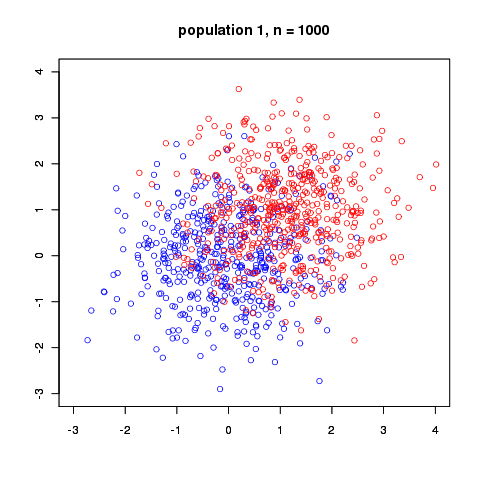
\includegraphics[height = 7cm, width = 7cm]{plots/exo1_simul_1.png}
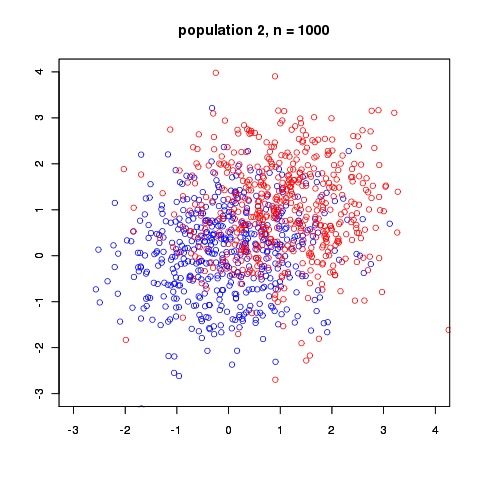
\includegraphics[height = 7cm, width = 7cm]{plots/exo1_simul_2.png}\\
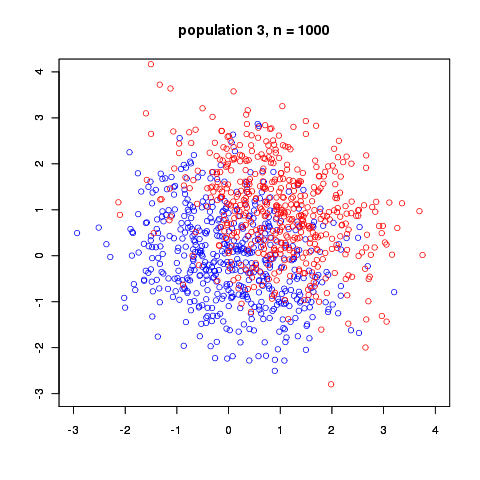
\includegraphics[height = 7cm, width = 7cm]{plots/exo1_simul_3.png}
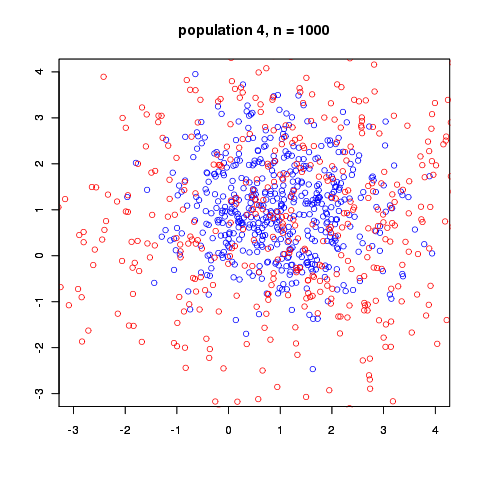
\includegraphics[height = 7cm, width = 7cm]{plots/exo1_simul_4.png}\\
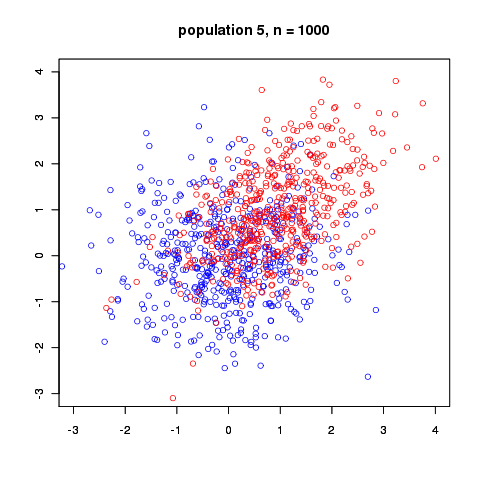
\includegraphics[height = 7cm, width = 7cm]{plots/exo1_simul_5.png}\\ \\
%TODO frontière de décision pour les 3 premiers cas.
Pour chaque cas de figure, nous avons déterminé l'expression d'un estimateur de la probabilité d'erreur,
ainsi que sa réalisation sur l'échantillon correspondant :\\
% TODO expression d'un estimateur de la probabilité d'erreur
Sa réalisation sur les échantillons nous donne les valeur suivantes :\\ \\
\begin{tabular}{|c|c|c|c|c|}
\hline
population & $\mu_{1}$ & $\mu_{2}$ & Erreur estimée ($\%$) & Erreur théorique ($\%$) \\
\hline
1 & (-0.028, -0.093) & (1.062, 0.981) & 27.6 & NA \\
\hline
2 & (0.346, 0.006) & (1.015, 0.982) & 31.1 & NA \\
\hline
3 & (-0.063, -0.045) & (1.036, 0.915) & 30.6 & NA \\
\hline
4 & (1.018, 0.919) & (1.221, 0.965) & 49 & NA \\
\hline
5 & (-0.127, -0.018) & (1.001, 1.002) & 28.2 & NA \\
\hline
\end{tabular}
$\\ \\$
Cela nous a permis de le comparer avec la probabilité d'erreur théorique.
% TODO probabilité d'erreur théorique

\newpage
\section*{Exercice 2 : Analyse discriminante sur les données \textit{Crabes}.}
Dans cet exercice, nous désirons utiliser l'analyse discriminante linéaire et l'analyse discriminante\\quadratique sur les données \textit{crabs}
afin de déterminer une fonction permettant de distinguer le sexe à partir des mesures \textit{FL} et \textit{RW}.\\

\subsection*{1. Expliquer ce que font les fonctions suivantes :}
\textbf{lda :} La fonction lda sert à effectuer l'analyse discriminante linéaire de données
(elle prend en paramètre une formule, un data frame ou une matrice).
Elle cherche à détecter si la matrice de covariance d'une classe est singulière.\\ \\
\textbf{qda :} Cette fonction est utilisée pour exécuter une analyse discriminante quadratique sur des données
en utilisant une décomposition QR qui retournera un message d'erreur si la variance du groupe est singulière pour chaque groupe.\\ \\
\textbf{contour :} Il s'agit d'une fonction générique utile pour créer un graphe de contour ou
pour ajouter des lignes de contour à un graphe existant.
Dans notre cas, elle est utile pour tracer les frontières de décision sur nos graphiques\\ \\
\textbf{sample :} Cette fonction nous permet de récupérer un échantillon de taille spécifiée d'éléments de l'ensemble X
en remettant en place ou non les éléments.\\ \\
\textbf{predict :} Predict() est une fonction générique de prédictions à partir des résultats des diverses fonctions de création de modèles.
La forme retournée dépend de la classe entrée en paramètre.\\ \\
\textbf{predict.lda :} Cette fonction classifie des observations multi-variables en utilisant l'analyse discrimante linéraire et
projette les données sur les discriminantes linéaires.
Cette fonction centre les discriminants linéaires de sorte que le nombre moyen pondéré des centres de gravité du groupe soit à l'origine.\\ \\
\textbf{Comparaison entre predict et predict.lda :} predict.lda() est une méthode de la fonction générique predict() pour la classe \textit{lda}.
On peut soit appeler predict() sur une classe lda d'un objet spécifié ou
appeler la fonction predict.lda() sans se soucier de la classe de l'objet.\\ \\

\subsection*{2. L'analyse discriminante quadratique et l'analyse discriminante linéaire des données \textit{crabs} :}
Nous avons d'abord effectué ces deux analyses sur les données \textit{crabs} en prenant comme échantillon d'apprentissage l'ensemble des données.\\
nous avons ensuite tracé les frontières de décision que nous avons obtenu (verte pour la lda et magenta pour la qda) :\\
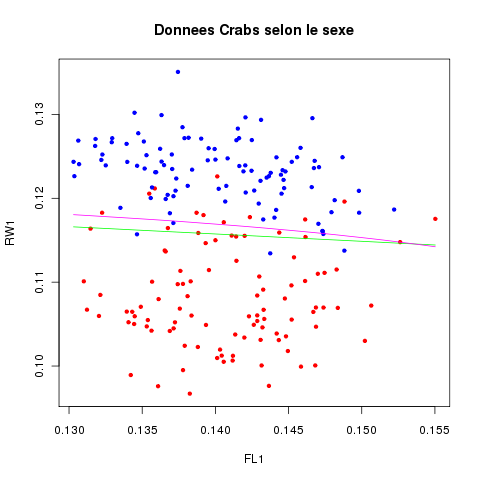
\includegraphics[height = 7cm, width = 7cm]{plots/exo2_analyse1.png}\\
Nous pouvons remarquer sur le graphique que les frontières de décision de chacune des deux analyses discriminantes sont sensiblement différentes,
et que certaines valeurs des données ne sont donc pas du même côté par rapport aux deux frontières.\\ \\
Nous avons donc calculé les estimations d'erreur sur cet échantillon d'apprentissage pour les deux\\analyses :\\ \\
\begin{tabular}{|c|c|}
\hline
Type d'analyse & Estimation d'erreur ($\%$) \\
\hline
lda & 9.5 \\
\hline
qda & 8.5\\
\hline
\end{tabular}\\
\textit{Ensemble d'apprentissage (la totalité des exemples)}\\ \\
Nous pouvons observer d'après ces deux valeurs que l'analyse discrimante linéaire semble moins précise que l'analyse discrimante quadratique
vu que la probabilité d'erreur pour la première est plus grande que la seconde.\\
Pour notre jeu de données, nous pouvons dire que les crabes ont sensiblement plus de chances d'être mieux classés avec l'analyse discrimante
quadratique qu'avec l'analyse discrimante linéaire.\\ \\

\subsection*{3. Estimation des erreurs de classification sur un ensemble d'apprentissage (2/3 des exemples au hasard)
et un ensemble de test (1/3 restants) :}
Dans un premier temps, nous nous sommes chargés de répartir aléatoirement les données \textit{crabs} afin d'obtenir nos échantillons
d'apprentissage et de test puis d'établir les probabilités d'erreur sur les\\analyses discriminantes quadratique et linéaires
sur les deux échantillons.\\ \\
Nous avons répété ces opérations 4 fois, ce qui nous donne les estimations d'erreur suivantes :\\ \\
\begin{tabular}{|c|c|c|c|c|}
\hline
\textbf{Ensemble d'apprentissage} & \multicolumn{4}{|c|}{Estimation d'erreur ($\%$)} \\
\hline
Type d'analyse & Éch n°1 & Éch n°2 & Éch n°3 & Éch n°4 \\
\hline
lda & 10.17 & 9.85 & 8.82 & 6.72 \\
\hline
qda & 7.63 & 7.58 & 7.35 & 8.4 \\
\hline
\end{tabular}\\
\textit{Ensemble d'apprentissage (2/3 des exemples au hasard)}\\ \\
Pour les échantillons d'apprentissage, nous pouvons remarquer que dans la majorité des cas,
l'analyse discriminante quadratique semble plus précise.
Cependant, dans notre dernier cas, l'analyse discriminante linéaire s'est montrée plus précise que la quadratique.\\ \\ \\
\begin{tabular}{|c|c|c|c|c|}
\hline
\textbf{Ensemble de test} & \multicolumn{4}{|c|}{Estimation d'erreur ($\%$)} \\
\hline
Type d'analyse & Éch n°1 & Éch n°2 & Éch n°3 & Éch n°4 \\
\hline
lda & 9.76 & 10.29 & 9.37 & 13.58 \\
\hline
qda & 8.54 & 8.82 & 7.81 & 8.64 \\
\hline
\end{tabular}\\
\textit{Ensemble de test (1/3 des exemples au hasard)}\\ \\
Pour la partie de test, il est possible aussi d'affirmer que l'analyse discrimante linéaire a plus de probabilité de faire des erreurs
dans la répartition des crabes dans les classes \textit{F} et \textit{M}.\\ \\
D'après la répétition du cacul des estimations de classification des crabes, nous pouvons dire que les deux analyses rangent les crabes
avec une estimation d'erreur quelque peu différentes.
L'analyse discrimante quadratique semble plus précise, comme vu dans la question précédente, que l'analyse discriminante linéaire,
mais il n'est pas possible de dire que cette dernière donnera forcément de moins bons résultats que la première.

\newpage
\subsection*{4. Répétition du calcul précédent en modifiant les proportions de\\découpage :}
\begin{tabbing}
Afin \= de répéter le calcul précédent en modifiant les proportions de découpage, nous avons choisi les proportions\\suivantes :\\
\> - 1/2 dans un premier temps.\\
\> - 4/5 dans un second temps.
\end{tabbing}
De plus, nous avons veiller à réaliser l'opération d'estimation d'erreur plusieurs fois pour obtenir diverses valeurs de probabilité :\\ \\
\begin{tabular}{|c|c|c|c|c|}
\hline
\textbf{Ensemble d'apprentissage} & \multicolumn{4}{|c|}{Estimation d'erreur ($\%$)} \\
\hline
Type d'analyse & Éch n°1 & Éch n°2 & Éch n°3 & Éch n°4 \\
\hline
lda & 11.96 & 10 & 6.36 & 6.25 \\
\hline
qda & 9.78 & 6.67 & 5.45 & 5.21 \\
\hline
\end{tabular}\\
\textit{Ensemble d'apprentissage (1/2 des exemples au hasard)}\\ \\
L'estimation des erreurs de classification pour ce cas rejoint les observations précédentes,
à savoir que l'analyse discriminante quadratique semble plus précise que l'analyse discriminante linéaire.\\ \\
\begin{tabular}{|c|c|c|c|c|}
\hline
\textbf{Ensemble de test} & \multicolumn{4}{|c|}{Estimation d'erreur ($\%$)} \\
\hline
Type d'analyse & Éch n°1 & Éch n°2 & Éch n°3 & Éch n°4 \\
\hline
lda & 6.48 & 8.18 & 11.11 & 9.61 \\
\hline
qda & 5.56 & 4.54 & 11.11 & 9.61 \\
\hline
\end{tabular}\\
\textit{Ensemble de test (1/2 des exemples au hasard)}\\ \\
Grâce à cet ensemble de test, il est possible de dire que dans certains cas, il y a autant de chances que l'analyse discriminante quadratique
soit assujettie aux mêmes erreurs de classification des éléments des données que l'analyse discriminante linéaire
(au vu des deux derniers échantillons).\\ \\
\begin{tabular}{|c|c|c|c|c|}
\hline
\textbf{Ensemble d'apprentissage} & \multicolumn{4}{|c|}{Estimation d'erreur ($\%$)} \\
\hline
Type d'analyse & Éch n°1 & Éch n°2 & Éch n°3 & Éch n°4 \\
\hline
lda & 11.51 & 10 & 10.71 & 7.36 \\
\hline
qda & 9.70 & 7.06 & 8.33 & 6.75 \\
\hline
\end{tabular}\\
\textit{Ensemble d'apprentissage (4/5 des exemples au hasard)}\\ \\
L'estimation des erreurs de classification pour cet ensemble d'apprentissage nous donne les mêmes observations que pour les cas précédents.\\ \\
\begin{tabular}{|c|c|c|c|c|}
\hline
\textbf{Ensemble de test} & \multicolumn{4}{|c|}{Estimation d'erreur ($\%$)} \\
\hline
Type d'analyse & Éch n°1 & Éch n°2 & Éch n°3 & Éch n°4 \\
\hline
lda & 0 & 3.33 & 6.25 & 8.11 \\
\hline
qda & 0 & 3.33 & 0 & 5.40 \\
\hline
\end{tabular}\\
\textit{Ensemble de test (1/5 des exemples au hasard)}\\ \\
Pour des groupes faibles d'éléments, les analyse discriminantes quadratique et linéaire peuvent avoir une probabilité d'erreur de classification
proche de zéro ou au contraire avoir une probabilité d'erreur proche de celle pour un grand nombre d'exemple
(le dernier échantillon tiré au hasard).\\ \\

\section*{Exercice 3 :}

\subsection*{}
\subsection*{}
\subsection*{}

\section*{Conclusion}

\end{document}
